\documentclass{bioinfo}
\copyrightyear{2015} \pubyear{2015}

\access{Advance Access Publication Date: Day Month Year}
\appnotes{Manuscript Category}
\RequirePackage{fixltx2e}

\begin{document}
\firstpage{1}

\subtitle{Subject Section}

\title[RNA-sequencing visualization]{Visualization methods for RNA-sequencing data analysis}
\author[Sample \textit{et~al}.]{Lindsay Rutter\,$^{\text{\sfb 1,}*}$, Adrienne N. Moran Lauter\,$^{\text{\sfb 2}}$, Michelle A. Graham\,$^{\text{\sfb 2,3}}$ and Dianne Cook\,$^{\text{\sfb 4,}*}$}
\address{$^{\text{\sf 1}}$Bioinformatics and Computational Biology Program, Iowa State University, Ames, IA 50011, USA, \\
$^{\text{\sf 2}}$USDA-ARS, Corn Insects and Crop Genetics Research Unit \\
$^{\text{\sf 3}}$Dept. of Agronomy, Iowa State University, Ames, IA 50010 \\
$^{\text{\sf 4}}$Econometrics and Business Statistics, Monash University, Clayton VIC 3800, Australia.}

\corresp{$^\ast$To whom correspondence should be addressed.}

\history{Received on XXXXX; revised on XXXXX; accepted on XXXXX}

\editor{Associate Editor: XXXXXXX}

\abstract{\textbf{Motivation:} Despite the availability of many ready-made testing software, reliable detection of differentially expressed genes in RNA-seq data is not a trivial task.  While the data collection might be considered high-throughput, data analysis has intricacies that require careful human attention. In light of this, researchers should use effective and modern data analysis techniques, and verify and enhance the appropriateness of their models with visual feedback. There is a need to make it easier for researchers to use models and visuals in a complimentary fashion during RNA-seq data analysis. \\
\textbf{Results:} We use several public RNA-seq data sets to show that our visualization tools can detect normalization issues, DEG designation problems, and common analysis errors. We also show that our visualization tools can identify genes of interest in ways undetectable with models. In this paper, we propose that users slightly modify their approach to RNA-seq analysis by incorporating statistical graphics into their usual analysis pipelines. \\
\textbf{Availability:} Interactive versions of graphics are available at shinyapps.io, as specified in the paper.\\
\textbf{Contact:} \href{lrutter@iastate.edu}{lrutter@iastate.edu}\\
\textbf{Supplementary information:} Supplementary data are available at \textit{Bioinformatics} online.}

\maketitle

\section{Introduction}

RNA-sequencing (RNA-seq) uses next-generation sequencing (NGS) to estimate the quantity of RNA in biological samples at given timepoints. In recent years, decreasing cost and increasing throughput has rendered RNA-seq an attractive form of transcriptome profiling. Prior to RNA-seq, gene expression studies were performed with microarray techniques, which required prior knowledge of reference sequences. RNA-seq does not have this limitation, and has enabled a new range of applications such as \textit{de novo} transcriptome assembly \citep{Robertson} and detection of alternative splicing processes \citep{Anders2012, Pan}. Coupled with its high resolution and sensitivity, RNA-seq has begun to revolutionize our understanding of the intricacies of eukaryotic transcriptomes \citep{Wang, Zhao}.

RNA-seq data is multivariate data, and its basic form is a matrix containing mapped read counts for \textit{n} rows of genes and \textit{p} columns of samples. These mapped read counts provide estimations of the gene expression levels across samples. Researchers typically conduct RNA-seq studies to identify differentially expressed genes (DEGs) between treatment groups. In most popular RNA-seq analysis packages, this objective is approached with models, such as the negative binomial model \citep{Anders2010, Trapnell2012, Trapnell2013, Robinson} and linear regression models \citep{Law}.

Initially, it was widely claimed that RNA-seq produced unbiased data that did not require sophisticated normalization \citep{Wang, Morin, Marioni}. However, numerous studies have since revealed that RNA-seq data is replete with biases and that accurate detection of DEGs is not a negligible task. Problems that complicate the analysis of RNA-seq data include nucleotide and read-position biases \citep{Hansen}, biases related to gene lengths and sequencing depths \citep{Oshlack, RobinsonOshlack}, biases introduced during library preparation \citep{McIntyre}, biases pertaining to the number of replications \citep{Schurch}, biases derived from overlapping sense-antisense transcripts and gene isoforms \citep{Trapnell2013}, and the confounding combination of technical and biological variability \citep{Bullard}.

In light of these complications, researchers should analyze RNA-seq data like they would any other biased multivariate data. Solely applying models to such data is problematic because models hold assumptions that must be verified to ensure statistical soundness. Fortunately, data visualization enables researchers to see patterns and problems they may not otherwise detect with traditional modeling. As a result, the most effective approach to data analysis is to iterate between models and visuals, and enhance the appropriateness of applied models based on feedback from visuals \citep{Shneiderman}. With RNA-seq data, we primarily want to compare the variability between replicates and between treatment groups. This is visually best achieved by drawing the mapped read count distributions across all genes and samples. Unfortunately, the few plotting tools offered in popular RNA-seq packages do not allow users to effectively view their data in this manner.

In this paper, we strive to remedy this problem by highlighting the utility of new and effective RNA-seq plotting tools. We use real RNA-seq data to show that our tools can detect normalization problems, DEG designation problems, and common errors in the analysis pipeline. We also show that our tools can identify genes of interest that cannot otherwise be obtained by models. We emphasize that interactive graphics should be an indispensable component of modern RNA-seq analysis: Researchers should be able to quickly flip through plots of genes that appear promising or problematic, and link between plots to swiftly obtain various perspectives of their data. Here, we do not propose that users drastically change their approach to RNA-seq analysis. Instead, we propose that users simply modify their approach to RNA-seq analysis by assessing the sensibility of their models with multivariate graphical tools, namely with parallel coordinate plots, scatterplot matrices, and litre plots.

\section{Parallel Coordinate Plots}

Parallel coordinate plots are essential to visually verify the relationships between variables in multivariate data. A parallel coordinate plot draws each row (gene) as a line. Connections between samples with positive correlations are flat, and connections between samples with negative correlations are crossed. The ideal dataset has more variability between treatments than between replicates. Researchers can quickly confirm this with a parallel coordinate plot: There should be flat connections between replicates but crossed connections between treatments.

There are several packages within the Bioconductor software that provide graphics for RNA-seq data analysis \citep{Huber}. Two of the most common graphic techniques are side-by-side boxplots and Multidimensional Scaling (MDS) plots \citep{Love, Risso, Robinson, Ritchie}. Unfortunately, these plots can hide problems that still exist in the data even after normalization and that could be better detected with parallel coordinate plots.

Figure~\ref{simulatedData} exemplifies this problem for two simulated datasets, one displayed on the left half and the other displayed on the right half of the figure. Each dataset contains two treatment groups (A and B) with three replicates. We cannot detect any notable differences between the left and right datasets from the side-by-side boxplots (subplots A) as they both show fairly consistent five number summaries across their six samples. Likewise, we cannot detect notable differences between the datasets from the MDS plots (subplots B) as they both suggest that the datasets are clustered by the two treatment groups, although the first replicate from treatment A appears as an outlier in the right MDS plot.

\begin{figure}
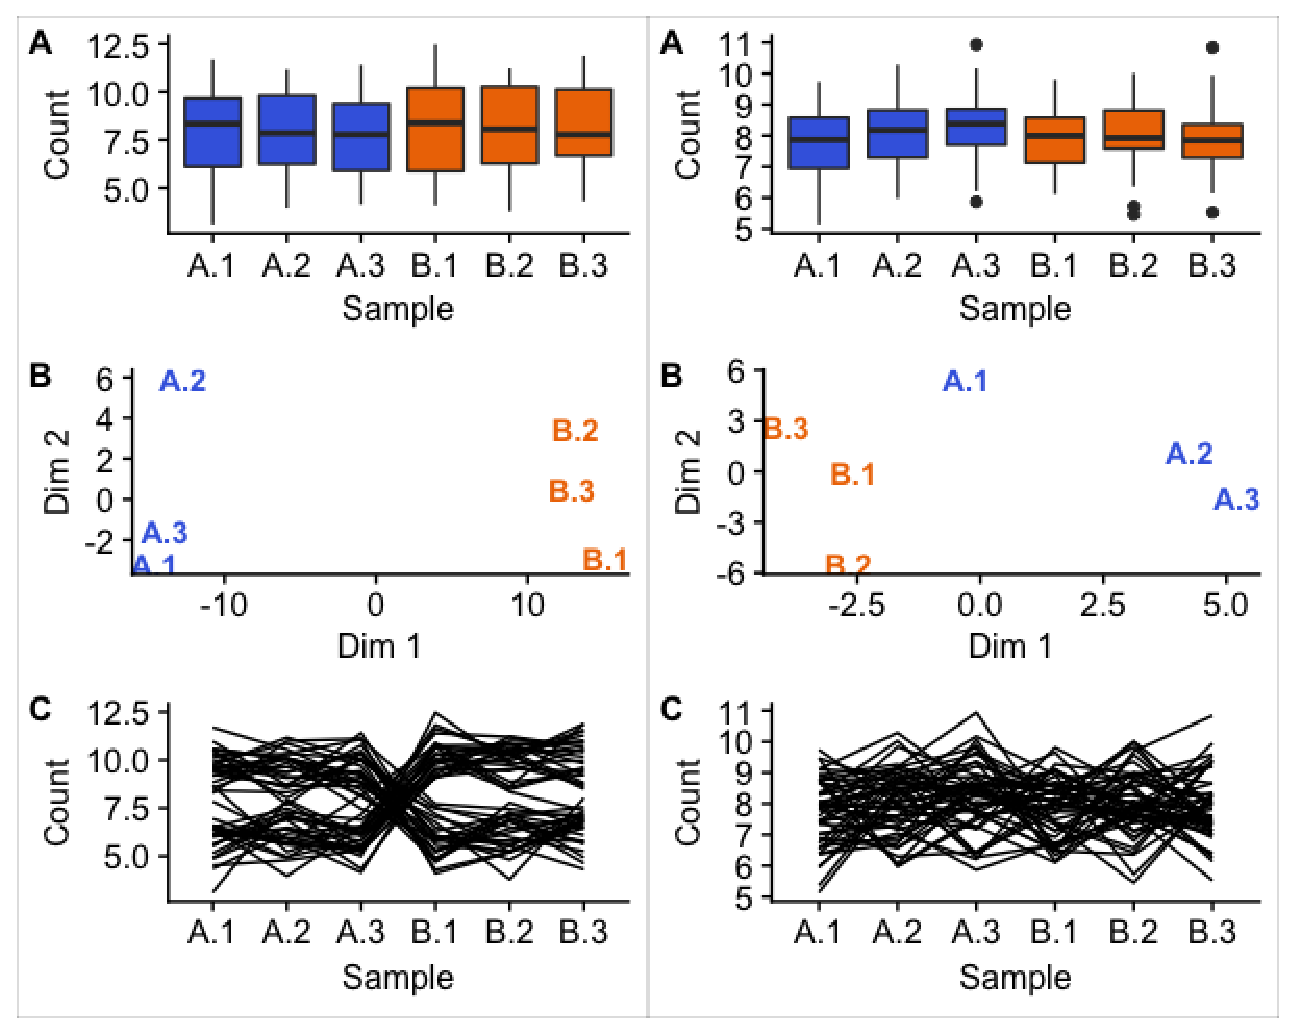
\includegraphics[width=\linewidth]{simulatedData.eps}
\caption{One simulated dataset is shown on the left half and another simulated dataset is shown on the right half of the figure. We do not see crucial distinctions between the left and right datasets with the boxplots (A subplots) and MDS plots (B subplots). However, the parallel coordinate plots (C subplots) show a critical difference between their structures. Namely, the left dataset is composed of genes with small replicate variation and large treatment group variation (suggesting DEGs), while the right dataset is composed of genes with similar variation between replicates and treatment groups (not suggesting DEGs). 
\label{simulatedData}}
\end{figure}

Despite this, we immediately see from the parallel coordinate plots (subplots C) that the left and right datasets have an important difference. The left dataset has consistent (level) lines between replicates and inconsistent (crossed) lines between treatment groups. This suggests that some of the genes (lines) have consistently low values for treatment group A and consistently high values for treatment group B, while some genes have the opposite phenomenon. As a result, these plotted genes may be DEG candidates. In contrast, the right dataset does not possess this ideal structure and suggests that the genes may not be DEG candidates. We could not see this important distinction using the side-by-side boxplots or the MDS plots because they only provide data summarization at the sample resolution, while the parallel coordinate plots show the sample connections for each of the 50 genes.

\begin{figure}
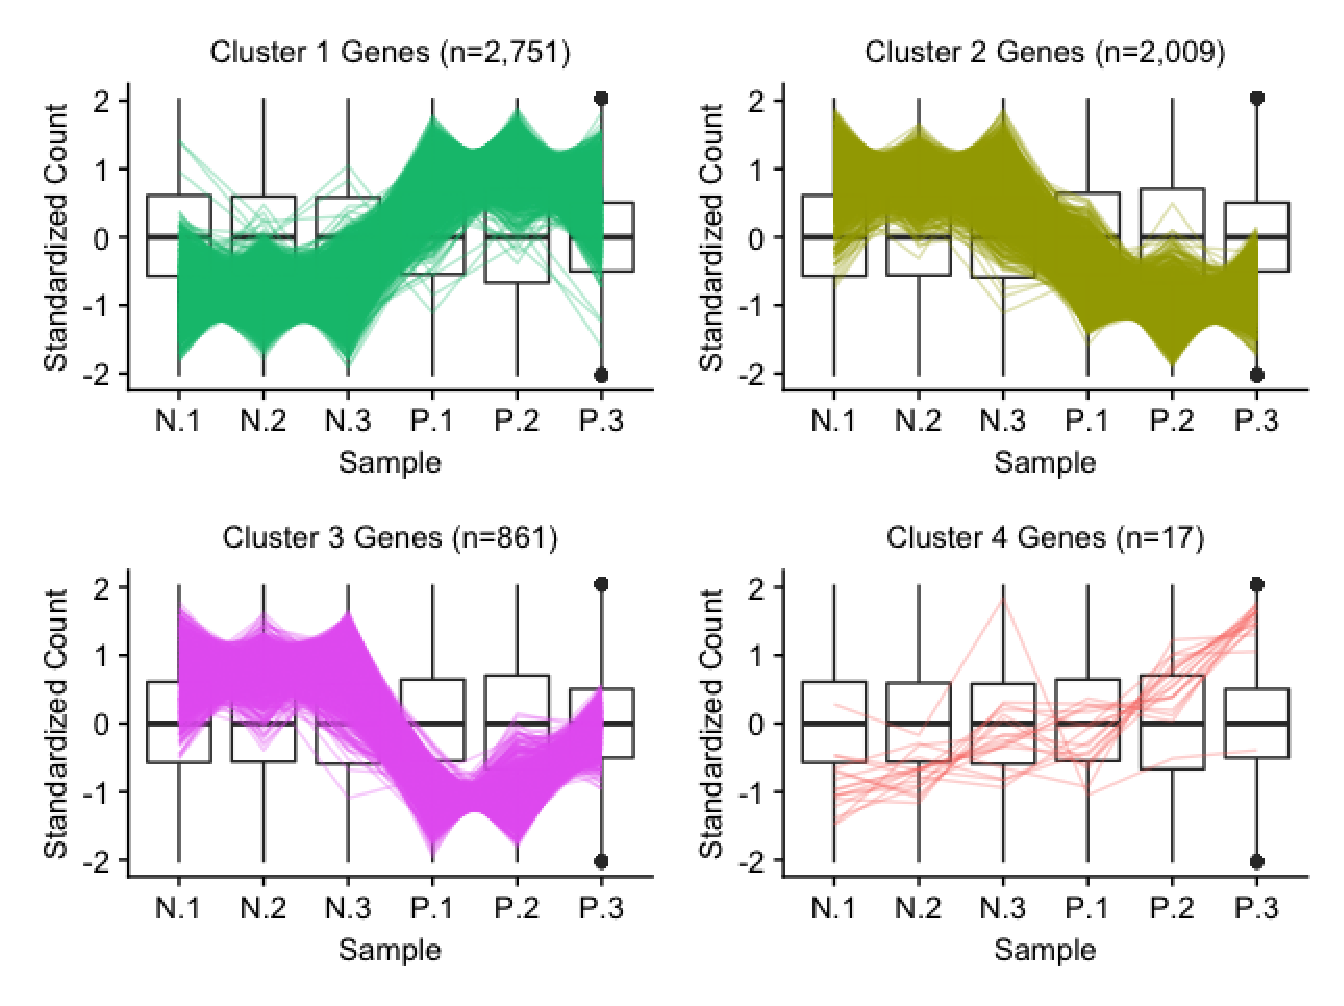
\includegraphics[width=\linewidth]{sbIRClustersSig.eps}
\caption{Parallel coordinate plots of significant genes after hierarchical clustering of the soybean iron metabolism data \citep{Lauter16}. We quickly confirm that Clusters 1 and 2 show the typical DEG pattern. Cluster 4 does not distinctively show the usual DEG pattern. Cluster 3 looks similar to Cluster 2, except for unexpectedly large P.3 values.
\label{sbIRClustersSig}}
\end{figure}

We will now examine the application of parallel coordinate plots to data from an RNA-seq study that compared soybean leaves after 120 minutes of iron-sufficient (group P) or iron-deficient (group N) hydroponic treatments \citep{Lauter16}. We filtered genes with low means and/or variance, performed a hierarchical clustering analysis with a cluster size of four, retained only significant genes, and visualized the results using parallel coordinate lines (Figure~\ref{sbIRClustersSig}). Supplementary Figure 1 shows the results before non-significant genes were removed. For these plots, we standardized each gene to have a mean of zero and standard deviation of unity \citep{Chandrasekhar, de Souto}.

The majority of significant genes were in Clusters 1 and 2, which for the most part captured the expected patterns of differential expression (consistent replicates and inconsistent treatments) in reverse directions. Only 17 significant genes belonged to Cluster 4 and they mostly showed messy patterns with low signal to noise ratios. Cluster 3 had a fairly large number of significant genes (n=861). These genes mostly showed clean differential expression profiles similar to Cluster 2 (large values for group N and small values for group P), except for unexpectedly large values for the third replicate of group P. The reasons for a different response by these genes on this replicate is unclear, but warrants further study.

\section{Scatterplot matrices}

\subsection{Overview of scatterplot matrices}

A scatterplot matrix is another effective multivariate visualization tool that plots read count distributions across all genes and samples. Specifically, it represents each row (gene) as a point in each scatterplot. With this method, users can quickly discover unexpected patterns, recognize geometric shapes, and assess the structure and association between multiple variables in a manner that is different from most common practices. 

\begin{figure}
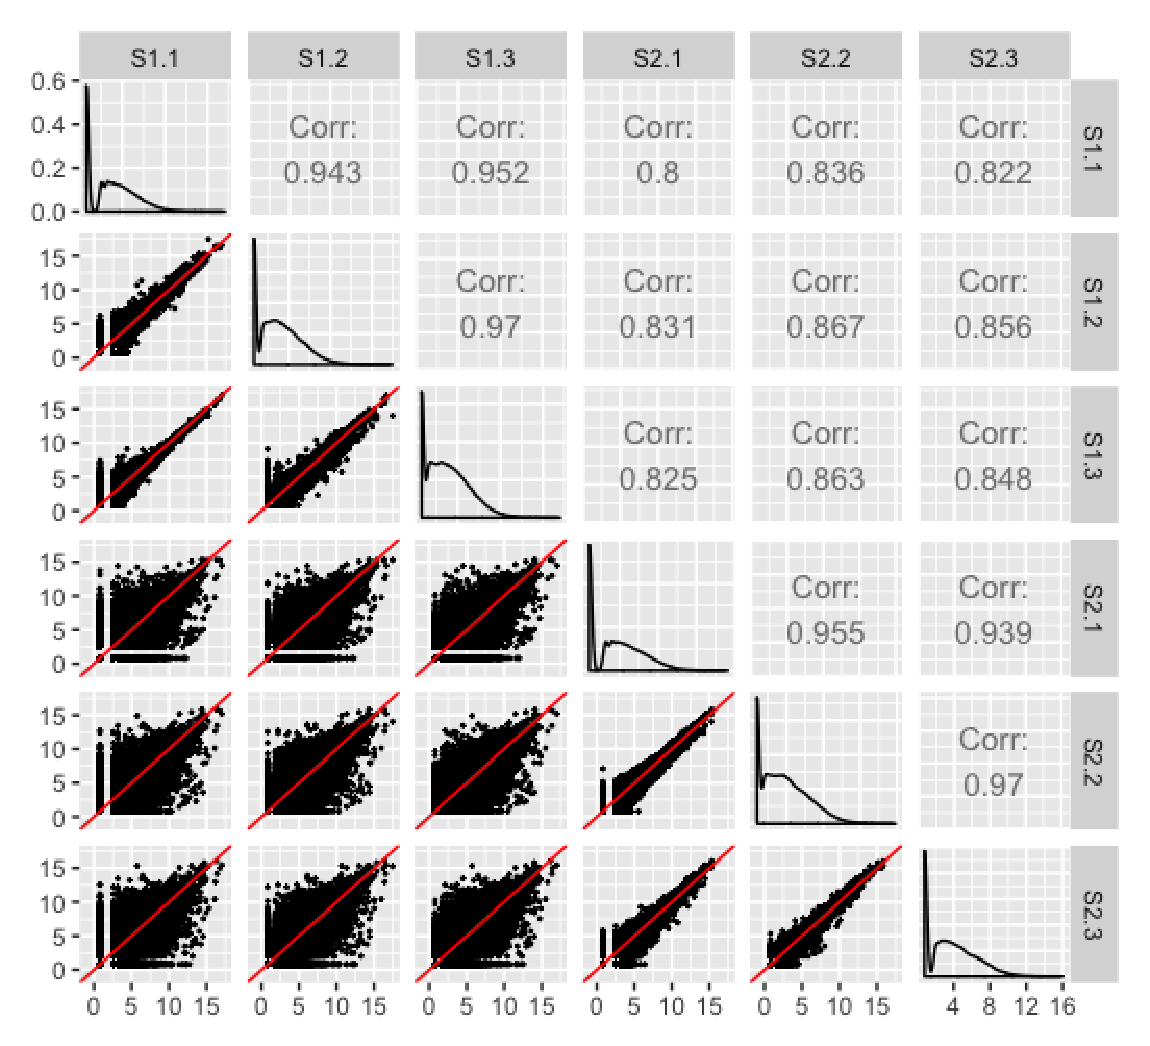
\includegraphics[width=\linewidth]{sbCNSM.eps}
\caption{Example of the expected structure of an RNA-seq dataset, using soybean cotyledon data from \cite{Brown}. Within a given scatterplot, most genes (points) should fall along the \textit{x=y} line. We should see genes deviate more strongly from the \textit{x=y} line in treatment scatterplots than in replicate scatterplots. 
\label{sbCNSM}}
\end{figure}

Clean data would be expected to have larger variability between treatment groups than between replicates. As Figure~\ref{sbCNSM} shows, researchers can quickly confirm this with a scatterplot matrix. Within each scatterplot, most genes should fall along the \textit{x=y} line (in red) as we expect only a small proportion of them to show differential expression between samples. However, a fraction of the genes should have lower variability between replicates than between treatments, and so we should expect the spread of the scatterplot points to fall more closely along the \textit{x=y} relationship between replicates than between treatments. Indeed, in Figure~\ref{sbCNSM}, we created a scatterplot matrix for a public RNA-seq dataset that contains three replicates for two developmental stages of soybean cotyledon (S1 and S2) \citep{Brown}. We can immediately verify that the nine scatterplots between treatment pairs (in the bottom-left corner of the matrix) have more spread around the \textit{x=y} line than the six scatterplots between replicate pairs.

After confirming this expected trend, users can use the scatterplot matrix to focus on subsets of genes: Outlier genes that deviate from the \textit{x=y} line in replicate scatterplots might be problematic, whereas outlier genes that deviate from the \textit{x=y} line in treatment scatterplots might be DEGs. In order to achieve this functionality, the plots must be rendered interactive.

Notice that each gene in our data is plotted once in each of the 15 scatterplots. With 73,320 genes in our data, more than one million points must be plotted. Rendering all points interactive would slow down the interactive capabilities of the plot. To solve this, we can tailor the geometric object of the scatterplots to be hexagon bins rather than points. This dramatically reduces the number of geometric objects to be plotted, and increases the interactivity speed.

The reader can visit https://rnaseqvisualization.shinyapps.io/scatmat to access the interactive version of Figure~\ref{sbIRClustersSig}. Readers can read the ``About" Tab to fully understand how to use the application. Essentially, the user can hover over a hexagon bin to see how many genes it contains. When the user clicks on a hexagon bin, the names of the genes are listed and superimposed as orange points across all scatterplots. The genes are also linked to a second plot that superimposes them as parallel coordinate lines on a side-by-side boxplot of all gene counts. This interactivity and linking allows users to quickly examine genes of interest from multiple perspectives superimposed onto the summary of all genes in the dataset.

\subsection{Assessing normalization with scatterplot matrices}

There is still substantial discussion about the normalization of RNA-seq data, and the scatterplot matrix can be used to understand and assess various algorithms. To exemplify this point, we will use a publicly-available RNA-seq dataset on Saccharomyces cerevisiae (yeast) grown in YP-Glucose (YPD) \citep{Risso}. The data contained four cultures from independent libraries that were sequenced using two library preparation protocols and either one or two lanes in a total of three flow-cells. This experimental design allowed researchers to examine various levels and combinations of technical effects (library preparation and protocol and flow cell) and biological effects (culture).

The four cultures (Y1, Y2, Y4, and Y7) were treated as biological replicates for which differential expression was not expected. Hence, the authors could establish a false positive rate in relation to the number of DEGs called between these groups. They then demonstrated that within-lane regression alone was insufficient in effectively removing biases. Instead, aggressive corrections for both within-lane (GC-content and gene length) and between-lane (count distribution and sequencing depth) biases were needed to effectively reduce the false-positive rate of DEG calls.

Figure~\ref{yeastWithinBetween}A shows the scatterplot matrix of the read counts from the Y1 and Y4 treatments after within-lane normalization. As we stated earlier, we expect most genes to show similar expression between samples, except for the handful that are differentially expressed. However, it is immediately clear that the data still was not sufficiently normalized as the distribution of genes is not centered around the \textit{x=y} lines. In contrast, Figure~\ref{yeastWithinBetween}B shows the scatterplot matrix of the read counts from the Y1 and Y4 treatments after \textit{both} within-lane and between-lane normalization, as was recommended by the authors due to its reduced false-positive rate. Indeed, the scatterplot matrix now follows the expected structure with most genes falling along the \textit{x=y} line with thicker deviations from it between treatment groups than between replicate groups.

Additionally, we can also confirm from Figure~\ref{yeastWithinBetween}B that the read counts fall closer to the \textit{x=y} line between the Y4 replicates (bottom-right scatterplot) than between the Y1 replicates (top-left scatterplot). This is expected because the Y1 replicates had additional technical variability as they used two different flow cells, whereas the Y4 replicates were from the same flow cell. As such, the scatterplot matrix can also be used to quickly inspect patterns of biological and technical variability in the dataset.

\subsection{Checking for common errors with scatterplot matrices}

Irreproducibility is prevalent in high-throughput biological studies. A study in Nature Genetics surveyed eighteen published microarray expression analyses and reported that only two were exactly reproducible \citep{Ioannidis}. The extent of the problem has spawned a field called ``forensic bioinformatics" whereby researchers attempt to reverse-engineer reported results back into the raw datasets simply to derive the methodologies used in published studies \citep{Baggerly}.

\begin{figure}
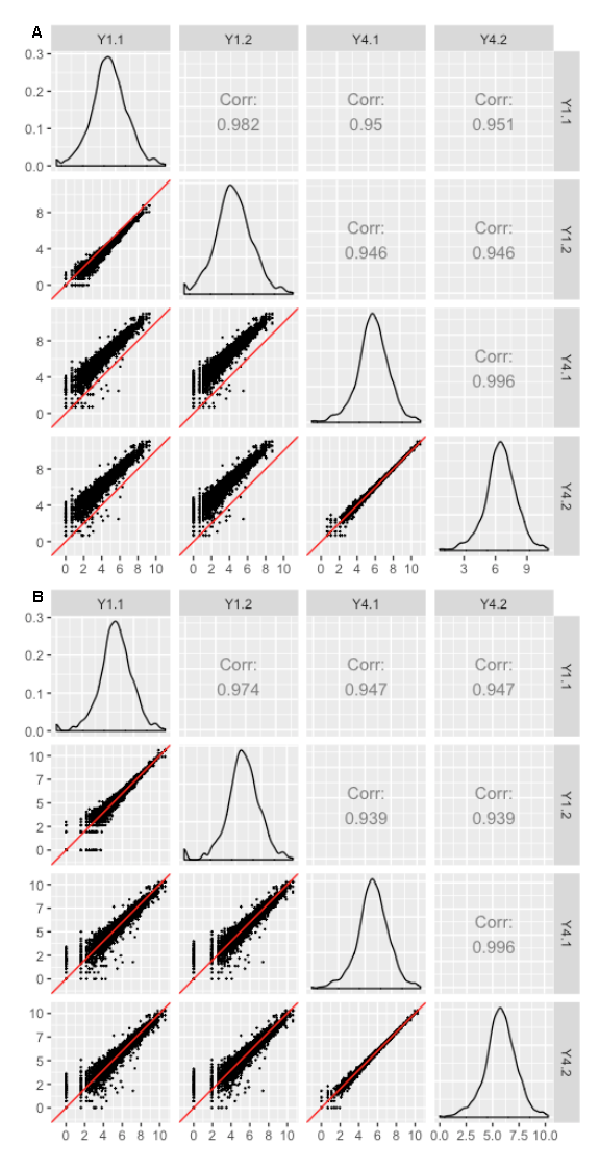
\includegraphics[width=\linewidth]{yeastWithinBetween.eps}
\caption{Illustrating normalization checks with data from \cite{Risso}. The collective deviation of genes from the \textit{x=y} line instantly reveals that the RNA-seq dataset was not thoroughly normalized using within-lane normalization (subplot A). However, within-lane normalization followed by between-lane normalization sufficiently normalized the data (subplot B). The authors who developed these normalization methods showed that the later approach generated a lower false-positive DEG call rate in this dataset.
\label{yeastWithinBetween}}
\end{figure}

Even though irreproducibility is merely cumbersome when it masks methods, it is unquestionably hazardous when it masks errors. With regards to personalized medicine, for example, obscured errors may cause well-intentioned researchers to present evidence for drugs that are ineffective or even harmful to patients \citep{Baggerly}. Forensic bioinformaticians who have actively investigated common errors in high-throughput biological studies have concluded that the largeness of the data itself may hinder our ability to detect errors \citep{Baggerly}. They also discovered that the most common errors are simple errors, such as mixing up sample labels \citep{Baggerly}. Collectively, these findings suggest that simple errors can be difficult to detect using common practices in high-throughput studies.

Fortunately, scatterplot matrices are a simple tool to check for common errors like sample mislabeling. Figure~\ref{sbCNSwitchedSM} shows the resulting scatterplot matrix after we deliberately swapped the labels of the third replicate of the first treatment group (S1.3) with the first replicate of the second treatment group (S2.1) in the previously-mentioned cotyledon dataset \citep{Brown}. We can immediately see that, as expected, there are nine scatterplots with thicker distributions around the \textit{x=y} line and six scatterplots with thinner distributions around the \textit{x=y} line. However, we notice that a subset of these thick and thin scatterplots appear outside of their expected locations given the expected variability between treatments versus replicates. Rearranging the columns of the two samples that appear suspicious in Figure~\ref{sbCNSwitchedSM} would indeed lead us back to the clean-looking scatterplot matrix we saw in Figure~\ref{sbIRClustersSig}. We cannot detect this mislabeling problem as convincingly with traditional plots, as can be verified with this dataset by comparing the boxplots and MDS plots before sample switching (left side of Supplementary Figure 2) and after sample switching (right side of Supplementary Figure 2).

\subsection{Finding unexpected patterns in scatterplot matrices}

Most popular RNA-seq plotting tools display summaries about the read counts, such as fold change summaries, principal component summaries, five number summaries, and dispersion summaries. In contrast to this trend, scatterplot matrices display the non-summarized read counts for all genes. This trait allows for geometric shapes and patterns relevant to the read count distribution to be readily visible in the scatterplot matrix.

An example of how geometric shapes in the scatterplot matrix can provide applicable information to researchers is shown in Figure~\ref{structure}, which uses the iron-metabolism soybean dataset \citep{Lauter16}. After normalizing the data, we see the expected pattern of a scatterplot matrix, with more variation around the \textit{x=y} line between treatments than between replicates (Figure~\ref{structure}).

However, one streak structure in the bottom right scatterplot stands out. A small subset of transcripts between replicates of the iron-sufficient group sharply deviates from the \textit{x=y} line. By interacting with the plot, we identified the five transcripts that deviated the most from the expected pattern, and searched for their putative functions. We discovered that these transcripts are reportedly involved in biotic and abiotic stress responses as well as the production of superoxides to combat microbial infections. It should be noted that these five transcripts did not reach significance unless the third replicate of the P group was removed.

Discussion with the authors of the study revealed that a lab biologist documented a clean data collection process. In the study, the authors aimed to determine the DEGs across three times points (30 minutes, 60 minutes, and 120 minutes) after exposure to the two iron condition levels. In order to reduce variability caused by plant handling by different researchers, the same researcher collected the samples in succession. One major finding from their study was a vast change in gene expression responses between these three time points (Supplementary Figure 3). In light of these discoveries, the authors tentatively suggest that the streak of genes shown in Figure~\ref{structure} may be due to the timing differences between replicate handling.

In any case, scientists cannot observe such interesting structures from any models. Hypothetically, these structures could lead to interesting post hoc analyses. For instance, if a similar structure presented itself in a dataset where the authors had noted an inadvertent experimental or biological discrepancy between those replicates, then a post hoc hypothesis that these genes might respond to that discrepant condition could be generated. Of course, this would only serve as a hypothesis generator; conventional genetic studies and additional evidence would be needed to confirm any possible role these genes have on this biological activity.

\begin{figure}
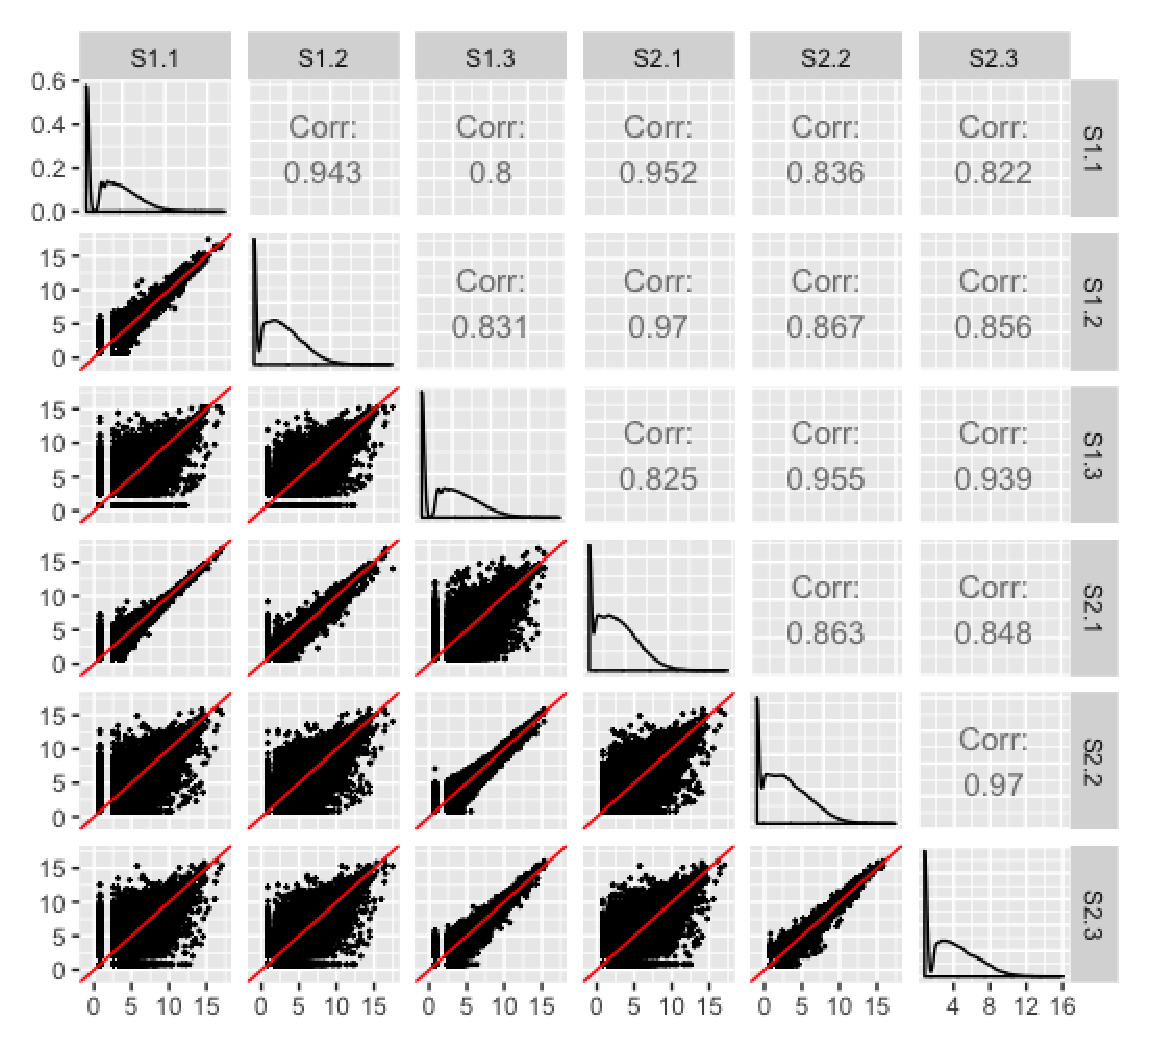
\includegraphics[width=\linewidth]{sbCNSwitchedSM.eps}
\caption{As expected, the scatterplot matrix of the coytledon data \citep{Brown} contains nine scatterplots with thicker distributions (should be treatment pairs) and six scatterplots with thinner distributions (should be replicate pairs). However, a subset of scatterplots unexpectedly show thicker distributions between replicate pairs and thinner distributions between treatment pairs. If we switch the labels of two suspicious samples (S1.3 and S2.1), the scatterplot matrix displays the anticipated structure we saw in Figure~\ref{sbCNSM}. At this point, we have evidence that these two samples may have been mislabeled, and we may wish to confirm this suspicion and correct it before continuing with the analysis.
\label{sbCNSwitchedSM}}
\end{figure}

\begin{figure}
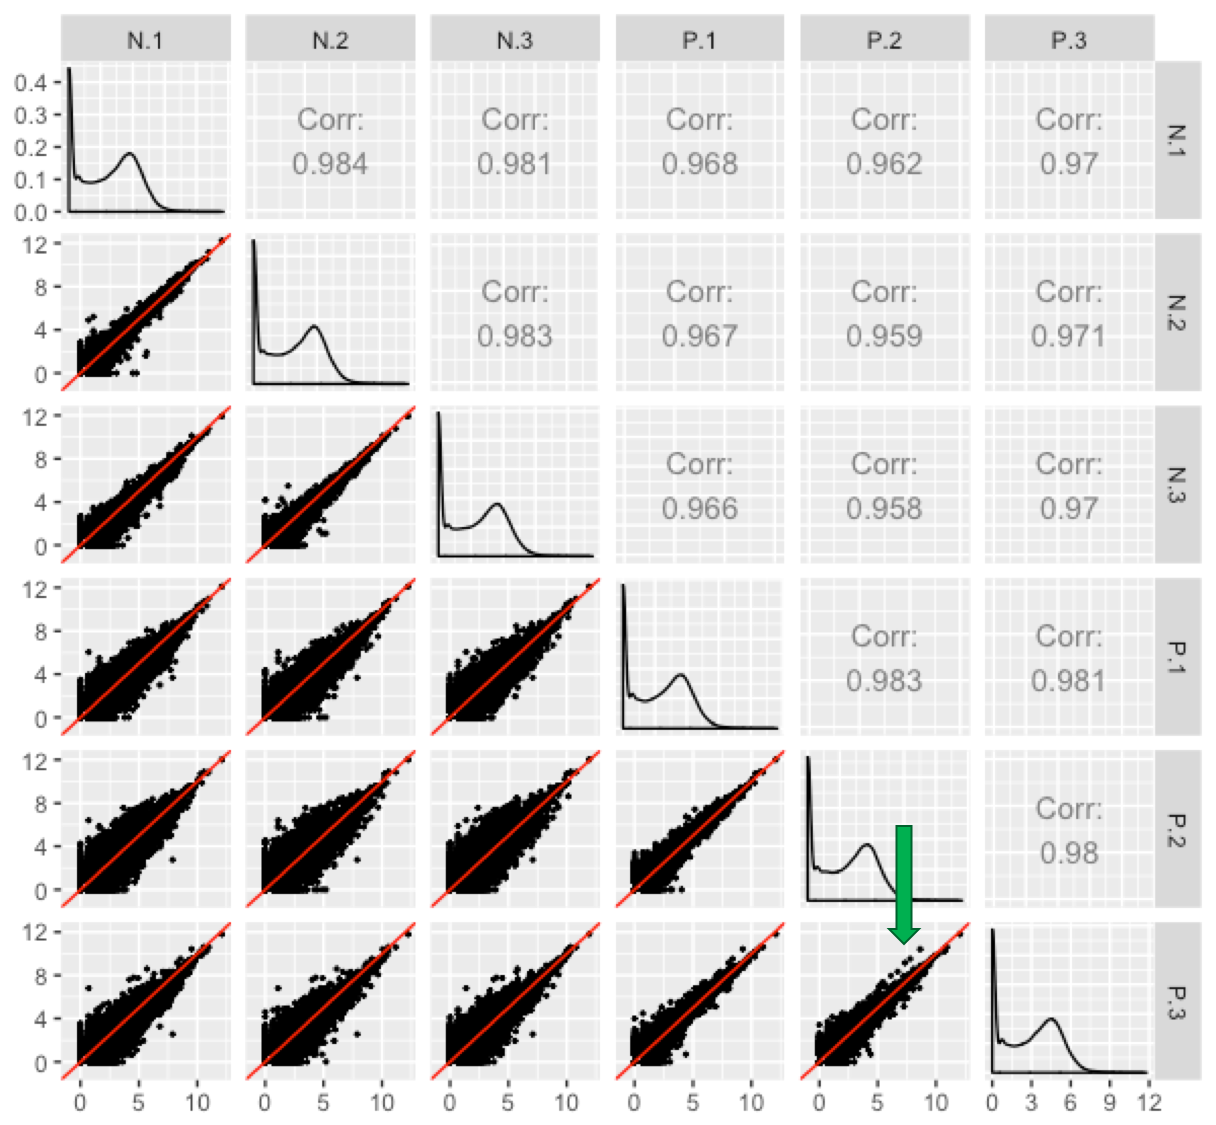
\includegraphics[width=0.98\linewidth]{sbIRStreak2.eps}
\caption{Scatterplot matrix of RNA-seq read counts from soybean leaves after exposure to iron-sufficient (treatment group P) and iron-deficient (treatment group N) hydroponic conditions~\citep{Lauter16}. We observe the expected structure of treatment pairs showing larger variability around the \textit{x=y} line than replicate pairs. However, we notice a pronounced streak structure in the bottom-right scatterplot (green arrow) that compares two replicate samples from the iron-sufficient group. The genes in the streak structure have large read counts that deviate in a parallel fashion from the \textit{x=y} line.
\label{structure}}
\end{figure}

\subsection{Assessing DEG calls in scatterplot matrices}

The scatterplot matrix can also be used to quickly examine the DEGs returned from a given model. Figure~\ref{sbIRDEG} shows the DEGs from the soybean cotyledon dataset superimposed as orange points onto the scatterplot matrix \citep{Brown}. We expect for DEGs to fall along the \textit{x=y} line for scatterplots between replicates and deviate from the \textit{x=y} line for scatterplots between treatment groups, as is confirmed in Figure~\ref{sbIRDEG}. As a side note, we can also link these DEGs as parallel coordinate lines on a side-by-side boxplot like in Figure~\ref{sbIRDEG} to confirm the expected pattern of differential expression from a second viewpoint. If we do not observe what should be expected of DEGs, then the DEG calls from the model may need to be scrutinized further.

As an additional example, we overlaid the significant genes from the four clusters of the iron-metabolism soybean dataset (originally shown in Figure~\ref{sbIRClustersSig}) onto the scatterplot matrix \citep{Lauter16}. The results are shown and briefly discussed in Supplementary Figures 4-7.

\section{Litre plots}

We demonstrated how to view differentially expressed genes onto the Cartesian coordinates of the scatterplot matrix in Figure~\ref{sbIRDEG}. Unfortunately, this figure becomes limited when we investigate treatment groups that contain a large number of replicates because we then have too many small scatterplots for it to remain an effective visualization tool. Moreover, researchers could benefit from additional plotting tools that allow them to quickly verify individual differentially expressed genes returned from a model. As a result, we developed a plot that allows users to visualize \textit{one} differentially expressed gene of interest onto the Cartesian coordinates of \textit{one} scatterplot matrix.

The ``replicate line plot" was developed by a group of researchers who demonstrated it could detect model scaling problems in microarray data \citep{Cook}. Unfortunately, this plot is only applicable on datasets where treatment groups contain exactly two replicates. The plot we now introduce is an extension of the ``replicate line plot" that can be applied to datasets with two or more replicates. We call this new plot a repLIcate TREatment (``litre") plot.

In the litre plot, each gene is plotted once for each possible combination of replicates between treatment groups. For example, there are nine ways to pair a replicate from one treatment group with a replicate from the other treatment group in the soybean iron-metabolism dataset (N.1 and P.1, N.1 and P.2, N.1 and P.3, N.2 and P.1, N.2. and P.2, N.2 and P.3, N.3 and P.1, N.3 and P.2, and N.3 and P.3) \citep{Lauter16}. Hence, each gene in this dataset is plotted as nine points in the litre plot. With 56,044 genes in this data, we would need to plot 504,396 points. This would reduce the speed of interactive functionality as well as cause overplotting problems. As a result, we again use hexagon bins to summarize this massive information (Figure~\ref{repDot} shows four example litre plots).

Once the background of hexagons has been drawn to give us a sense of the distribution of all treatment pair combinations for all genes, the user can superimpose the nine points of one gene of interest. We can examine and compare litre plots using the clusters we created in Figure~\ref{sbIRClustersSig}. Subplots A and B of Figure~\ref{repDot} each show a significant gene from Cluster 2 plotted as nine mustard points, subplots C and D each show a significant gene from Cluster 3 plotted as nine pink points, and subplots E and F each show a significant genes from Cluster 4 plotted as nine coral points. Note that, in the examples in Figure~\ref{repDot}, the read counts of treatment pair combinations sometimes overlap, resulting in the appearance of less than nine points being overlaid. Example litre plots from Cluster 1 are shown in Supplementary Figure 8.

\begin{figure}
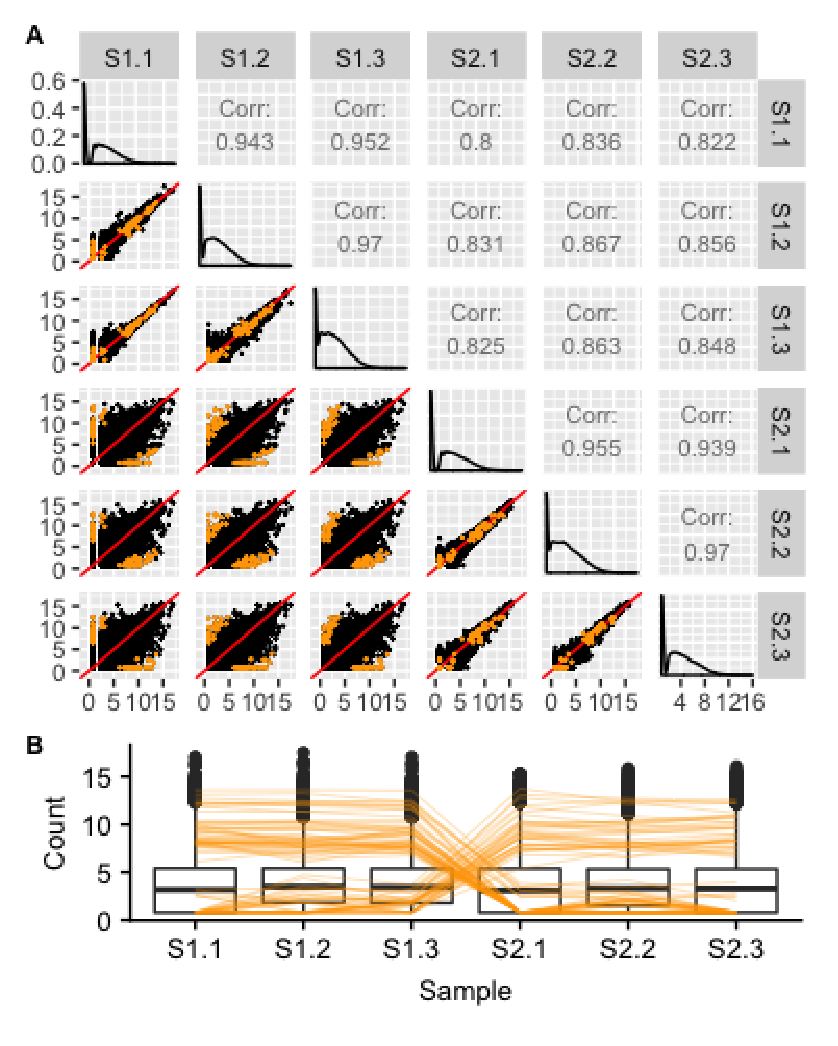
\includegraphics[width=\linewidth]{sbIRDEG.eps}
\caption{Example of the expected structure of DEG calls (in orange) from the soybean cotyledon dataset \cite{Brown}. In the scatterplot matrix (subplot A), DEGs should fall along the \textit{x=y} line for replicates and deviate from it for treatments. In the parallel coordinate plot (subplot B), DEGs should show levelness between replicates and crosses between treatments. These two plotting types can be linked to quickly provide users multiple perspectives of their DEG calls.
\label{sbIRDEG}}
\end{figure}

\begin{figure}
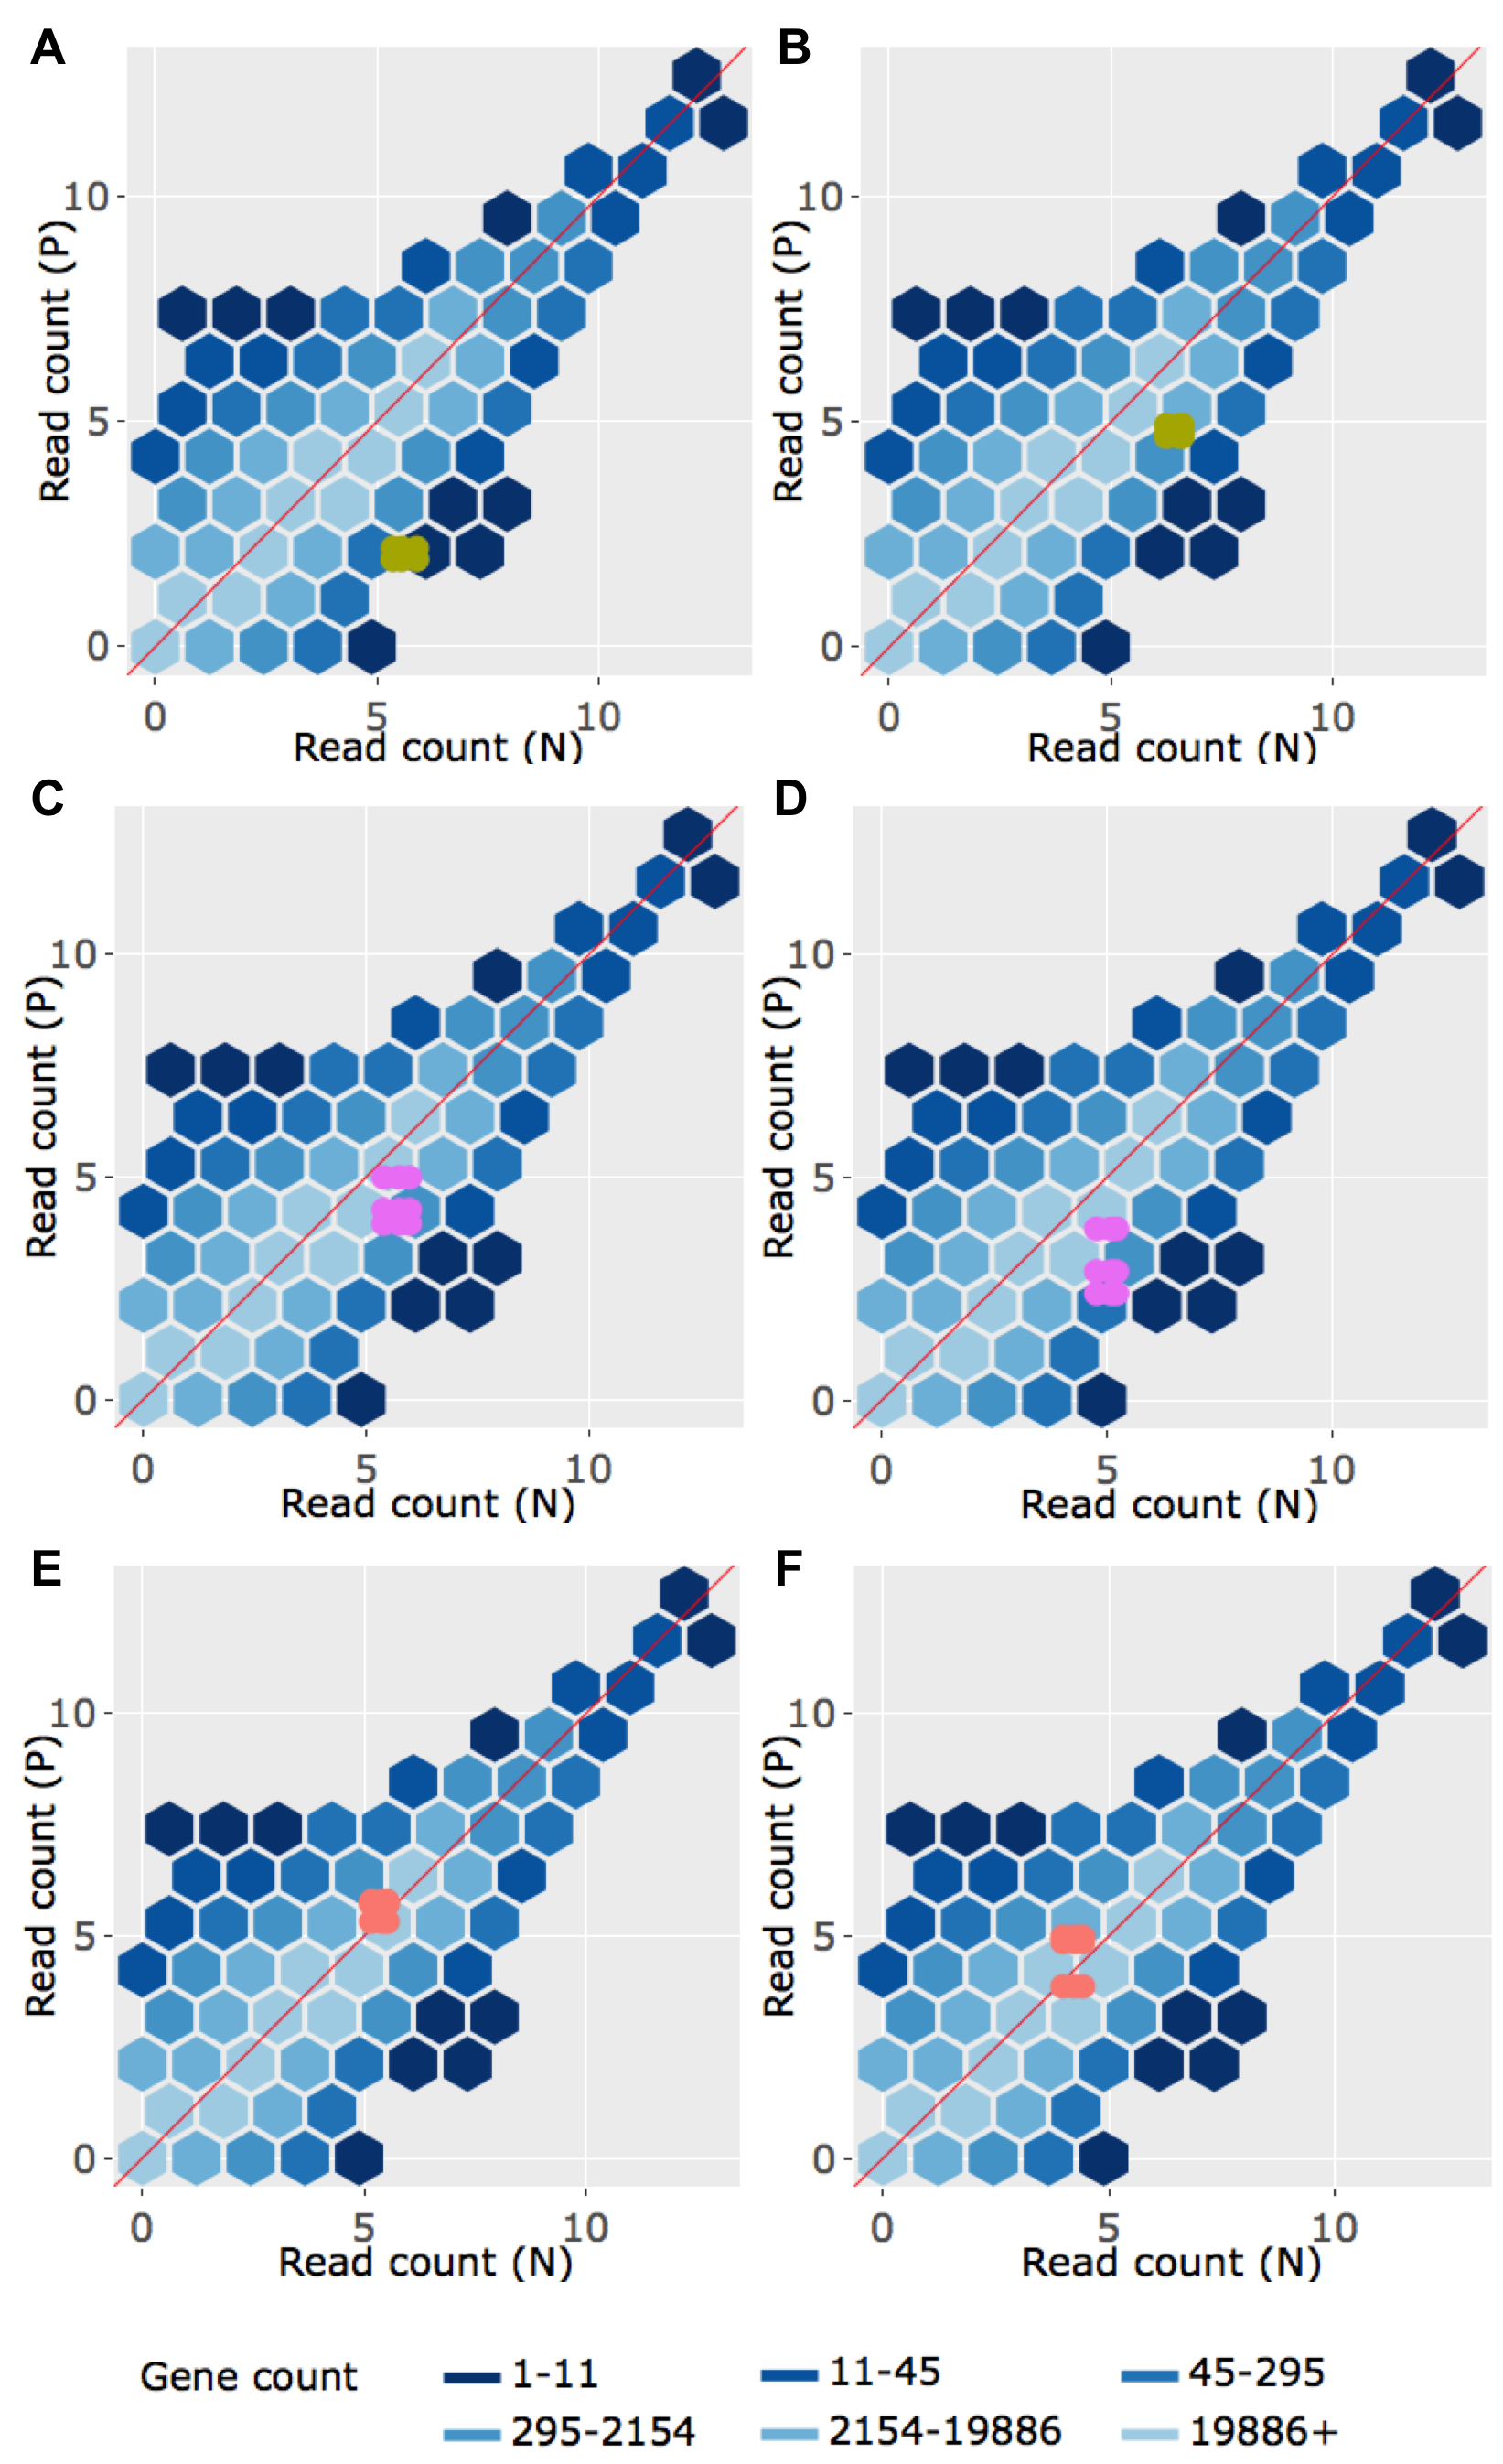
\includegraphics[width=\linewidth]{litre6LB.eps}
\caption{Litre plots for representative genes from clusters created in Figure~\ref{sbIRClustersSig} \citep{Lauter16}. Subplots A and B each show a gene from Cluster 2 overlaid as nine mustard points. Subplots C and D each show a gene from Cluster 3 overlaid as nine pink points. Subplots E and F each show a gene from Cluster 4 overlaid as nine coral points. Litre plots allow us to quickly flip through genes and search for (possibly odd) patterns that may not be detected numerically.
\label{repDot}}
\end{figure}

For the case of Figures~\ref{repDot} A and B, the nine overlaid points are superimposed in a manner we would expect from a differently expressed gene: They are located far from the \textit{x=y} line (difference between treatments) and are close to each other (similarity between replicates). In fact, the replicates in subplot B are so precise that the overlaid points almost entirely overlap each other. In contrast, Figures~\ref{repDot} C and D do not seem to show as much replicate consistency. Now, there seems to be a pattern in which one replicate from the P group is larger than (and visually distanced from) the other two replicates. In other words, litre plots are able to capture the pattern differences in the significant genes from Cluster 2 and 3 that we saw back in Figure~\ref{sbIRClustersSig}.

Moreover, in the case of Figures~\ref{repDot} E and F, the nine overlaid points are not clearly superimposed in the distinct pattern we expect of significant genes. While subplot E shows a gene that has consistent replications, the difference between the treatment groups is so small that the overlaid points cluster around the \textit{x=y} line. Additionally, the gene displayed in subplot F shows inconsistent replications and consistent treatment groups, as the spread-out overlaid points center on the \textit{x=y} line. Despite these genes being deemed significant by the model, the litre plots call into question whether the genes from this cluster show an expected profile of differential expression. This is similar to the messy-looking parallel coordinate plots we saw from these genes in Cluster 4 back in Figure~\ref{sbIRClustersSig} and the messy-looking superimposition we saw from these genes in Cluster 4 onto the scatterplot matrix in Supplementary Figure 7. As a result, litre plots can detect odd and questionable patterns in individual ``significant genes" that cannot be detected numerically through models. If this happens, the user may wish to further investigate these DEG calls.

The interactive litre plots for Cluster 2 DEGs (Figure~\ref{repDot} A and B), Cluster 3 DEGs (Figure~\ref{repDot} C and D), and Cluster 4 DEGs (Figure~\ref{repDot} E and F) are available at https://rnaseqvisualization.shinyapps.io/litreCluster\#, where \# is 2, 3, or 4, respectively. As can be verified in these interactive versions, users are provided several input fields that tailor the plot functionality. For instance, the user may wish to quickly scroll through significant genes one by one in order of increasing FDR values. Please read the ``About" tab in the interactive links for more information.

\section{Closing case study}

We briefly discuss an additional example that merges many of the topics addressed in this paper. The publicly available data for this example contain technical replicates of liver and kidney RNA samples from one human male \citep{Marioni}. We first calculate DEG calls for this data using the popular normalization method of library size scaling, where the number of total reads in each sample are normalized to a common value across all samples. This process leads to 9,018 DEGs, with most of them ($\sim$78\%) showing higher expression in the kidney group.

Although we could finish our analysis at this point and draw conclusions based on this list of DEGs that came from the model, it would be wise to also view this dataset visually. Viewing this data as a scatterplot matrix confirms the expected pattern with treatment scatterplots showing larger variation than technical replicate scatterplots. However, it also uncovers a hidden pattern in the treatment plots: There is a pronounced streak of genes with higher expressions in the liver group (Figure~\ref{lkSM}). We should also view the DEGs from the model using parallel coordinate plots: Upon doing so, we notice that while the 1,968 liver-specific DEGs follow the expected pattern of significant calls, a substantial fraction of the 7,050 kidney-specific DEGs appear comparatively noisy (Figure~\ref{lkClusters}A).

\begin{figure}
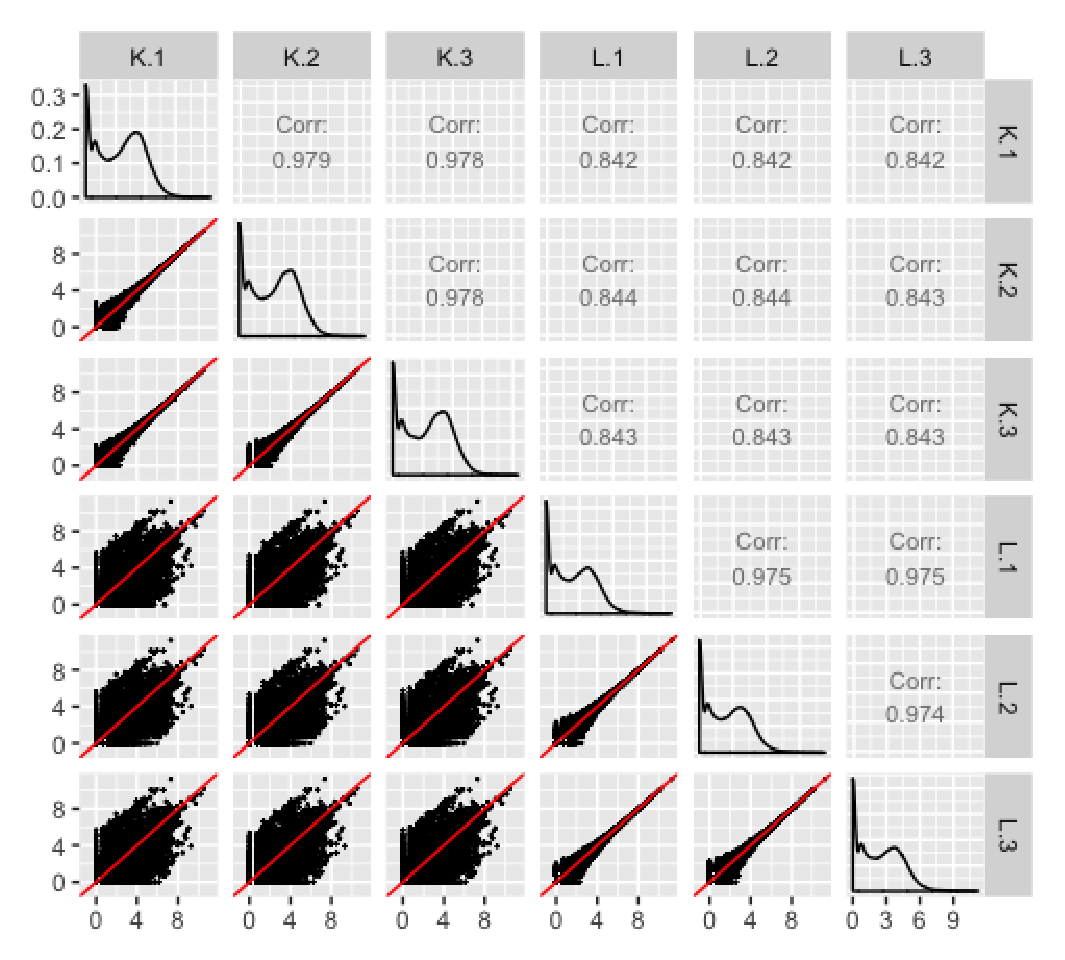
\includegraphics[width=1\linewidth]{lkSM.eps}
\caption{Scatterplot matrix of liver and kidney technical replicates \citep{Marioni}. The technical replicate scatterplots look precise as is expected, with little variability around the \textit{x=y} line. The treatment group scatterplots have much more variability around the \textit{x=y} line, as we would expect. However, each treatment group scatterplot contains a pronounced streak of highly-expressed liver-specific genes, which deviates from the expected distribution. Some researchers have suggested that differences in the distribution of reads between groups may require particularly stringent normalization.
\label{lkSM}}
\end{figure}

Taking both of these observations into account, we may need to reconsider our normalization technique. Some authors have argued that the popular library scaling method is not adequate in all cases, especially when the underlying distribution of reads between samples is inconsistent. In the current data, the observed streak of outlier genes that are highly expressed in the liver samples reduces the sequencing quota available to the remaning genes in these samples, which could create an articial inflation of the kidney-specific DEG calls. These authors have recommended TMM normalization for such cases (including for this particular dataset) as this technique generates sample scaling factors that consider sample distributions \citep{RobinsonOshlack}.

In light of all this, we return to square one and now apply TMM normalization to this data. This process leads to 7,520 DEGs that have a more level distribution between the kidney ($\sim$53\%) and liver ($\sim$47\%) groups. The scatterplot matrix did not appear differently from what we saw in Figure~\ref{lkSM} as both of these normalization methods are scaling procedures. However, we should visualize the new DEG calls. Plotting these DEGs as parallel coordinate lines paints a much cleaner picture from what we saw earlier, with most genes following the expected pattern of significance (Figure~\ref{lkClusters}B). Of the 7,050 kidney-specific DEGs we saw previously with library scaling normalization, only a cleaner-looking subset (n=3,974) of them remained as such using TMM normalization.

\begin{figure}
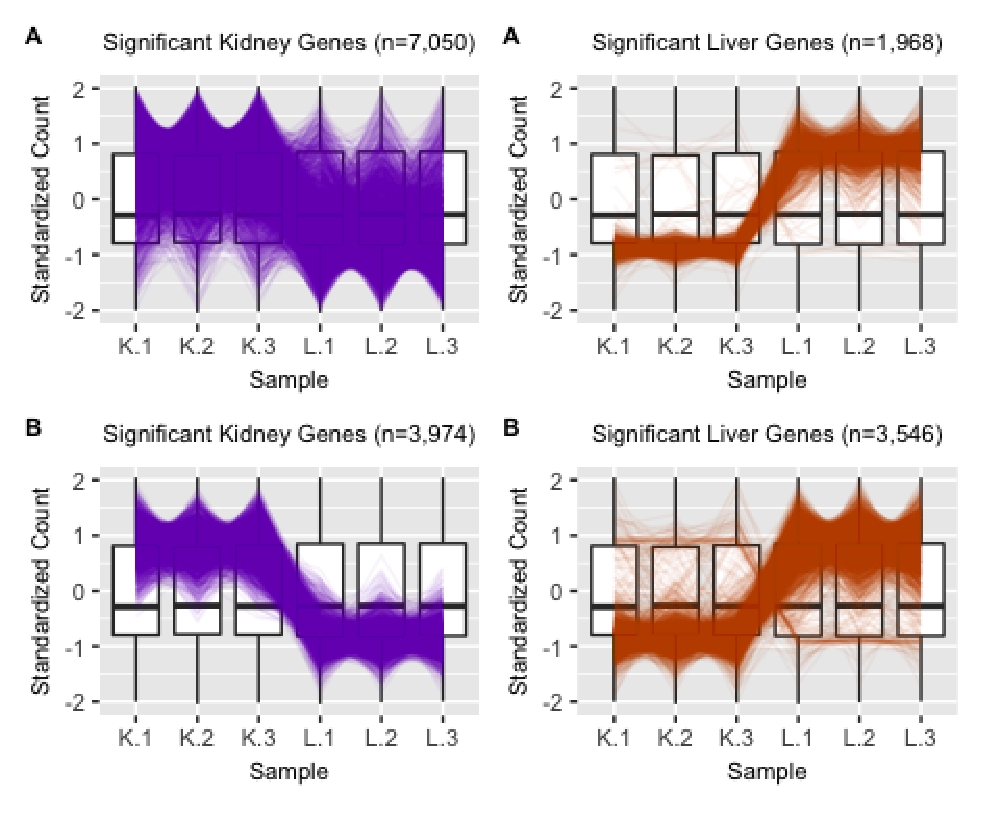
\includegraphics[width=1\linewidth]{lkClusters.eps}
\caption{Subplot A shows parallel coordinate plots of the DEGs from liver and kidney technical replicates \citep{Marioni} after standard library scale normalization. The division of DEGs between the two groups was rather disparate, with ~78\% of the DEGs being kidney-specific and only ~22\% of the DEGs being liver-specific. Also of note, while the parallel coordinate patterns of the liver-specific DEGs appear as expected, the patterns of the kidney-specific DEGs seem to show comparatively larger variability between the replicates. Subplot B shows parallel coordinate plots of the DEGs from liver and kidney technical replicates after TMM normalization. The division of DEGs between the two groups is more balanced, with ~53\% of the DEGs being kidney-specific and ~47\% of the DEGs being liver-specific. Additionally, the parallel coordinate patterns of both the liver-specific and kidney-specific DEGs appear as expected and more consistent with each other.
\label{lkClusters}}
\end{figure}

A deeper investigation of the effects of normalization on this data are shown in the supplementary material. These plots collectively suggest that this datasest indeed requires more than just library scaling for reliable analysis. This case study was meant to underscore the overarching theme of this paper that iteration between models and visualizations is crucial to achieve the most convincing results and conclusions in RNA-seq studies.

\section{Discussion}

In this paper, we strived to convince readers that effective visualization should be a crucial part of RNA-seq analysis. We used real data to demonstrate that scatterplot matrices, parallel coordinate plots, and litre plots help users check for normalization problems, catch common errors in analysis pipelines, and confirm that the variation between replicates and treatments is as expected. We also showed that these graphical tools allow researchers to quickly explore DEG lists that come out of models and ensure which ones make sense from an additional and arguably more intuitive vantage point. Moreover, we demonstrated that our simple plotting tools allow researchers to discover genes of interest through visual geometric patterns that would otherwise remain undiscovered with models.

In general, scientists might uncover surprising patterns lurking in their data with plots in ways that cannot be achieved with any formulas or models. Researchers from all statistical backgrounds can use graphical tools to better understand (if not demystify) how the application of various normalization techniques and/or models affect their results. All in all, scientists can gain more confidence in the data analysis pipelines they choose and in the results they draw at the mere cost of briefly creating and exploring graphical outputs during their analyses.

Modern data analysis is most reliable when models and visuals are used congruently. Unfortunately, the current culture around RNA-seq analysis de-emphasizes the importance of graphical tools, which, as we have shown, calls into question the soundness of results that come from RNA-seq studies. Solving this problem is straightforward and does not require scientists to drastically change their approach to RNA-seq analysis. Instead, scientists simply need to incorporate effective plotting tools during their usual analysis pipelines. We plan to serve a role in this solution by publishing a new \textsf{R} software package that includes the useful plotting techniques we introduced in this paper. To encourage scientists to use this resource, we aim to include a straight-forward vignette that demonstrates how to painlessly apply these graphical tools to RNA-seq data. It is our hope that such work will serve a small part in upgrading the RNA-seq analysis world into one that more wholistically extracts meaningful biological information using both models and visuals.

\section*{Acknowledgements}

R \citep{R} was used to conduct analyses in this paper. Packages ggplot2 \citep{ggplot2}, shiny \citep{shiny}, plotly \citep{plotly}, and htmlwidgets were used to build the graphics. 

\section*{Funding}

Research of Graham and Moran Lauter was financed by the United States Department of Agriculture, Agricultural Research Service (USDA-ARS) CRIS Project 5030-21220-005-00D and the Iowa Soybean Association.

\begin{thebibliography}{}

% Shu reference --> Glimma
% Marini reference --> pcaExplorer
% htmlwidgets --> htmlwidgets

\bibitem[Anders and Huber, 2010]{Anders2010}
Anders, S. and Huber, W. (2010) Differential expression analysis for sequence count data, {\it Genome Biology}, {\bf 11}, R106.

\bibitem[Anders {\it et~al}., 2012]{Anders2012}
Anders, S., Reyes, A., and Huber, W. (2012) Detecting differential usage of exons from RNA-seq data. {\it Genome Research}, {\bf 22}, 2008--2017.

\bibitem[Baggerly and Coombes, 2009]{Baggerly}
Baggerly, K.A. and Coombes, K.R. (2009) Deriving chemosensitivity from cell lines: Forensic bioinformatics and reproducible research in high-throughput biology. {\it The Annals of Applied Statistics}, {\bf 3}, 1309--1334.

\bibitem[Brown and Hudson, 2015]{Brown}
Brown, A.V. and Hudson, K.A. (2015) Developmental profiling of gene expression in soybean trifoliate leaves and cotyledons. {\it BMC Plant Biology}, {\bf 15}, 169.

\bibitem[Bullard {\it et~al}., 2010]{Bullard}
Bullard, J. H., Purdom, E., Hansen, K. D., and Dudoit, S. (2010) Evaluation of statistical methods for normalization and differential expression in mRNA-Seq experiments. {\it BMC Bioinformatics}, {\bf 11}, 94.

\bibitem[Chandrasekhar {\it et~al}., 2011]{Chandrasekhar}
Chandrasekhar, T., Thangavel, K., and Elayaraja, E. (2011) Effective clustering algorithms for
gene expression data. {\it International Journal of Computer Applications}, {\bf 32}, 4.

\bibitem[Chang  {\it et~al}., 2017]{shiny}  
Chang, W., Cheng, J., Allaire, JJ, Xie, Y. and McPherson, J. (2017). {\it shiny: Web application framework for R}, R package version 1.0.5. https://CRAN.R-project.org/package=shiny

\bibitem[Cook {\it et~al}., 2007]{Cook}
Cook, D., Hofmann, H., Lee, E.-K., Yang, H., Nikolau, B., and Wurtele, E. (2007) Exploring gene expression data, using plots. {\it Journal of Data Science}, {\bf 5}, 151--182.

\bibitem[de Souto {\it et~al}., 2008]{de Souto}
de Souto, M.C.P, de Araujo, D.S.A, Costa, I.G., Soares, R.G.F., Ludermir, T.B., and Schliep, A. (2008) Comparative study on normalization procedures for cluster analysis of gene expression datasets. {\it International Joint Conference on Neural Networks}, 2793--2799.

\bibitem[Hansen {\it et~al}., 2010]{Hansen}
Hansen, K.D., Brenner, S.E., and Dudoit, S. (2010) Biases in Illumina transcriptome sequencing caused by random hexamer priming. {\it Nucleic Acids Research}, {\bf 38}, e131.

\bibitem[Huber {\it et~al}., 2015]{Huber}
Huber, W., Carey, V.J., Gentleman, R,, Anders, S,, Carlson, M., and Carvalho, B.S. (2015) Orchestrating high-throughput genomic analysis with Bioconductor. {\it Nature Methods}, {\bf 12}, 115--121.

\bibitem[Ioannidis {\it et~al}., 2009]{Ioannidis}
Ioannidis, J.P., Allison, D.B., Ball, C.A., Coulibaly, I., Cui, X., Culhane, A.C., Falchi, M., Furlanello, C., Game, L., Jurman, G., Mangion, J., Mehta, T., Nitzberg, M., Page, G.P., Petretto, E. and van Noort, V. (2009) Repeatability of published microarray gene expression analyses. {\it Nature Genetics}, {\bf 41}, 149--155.

\bibitem[Law {\it et~al}., 2014]{Law}
Law, C.W., Chen, Y., Shi, W., and Smyth, G.K. (2014) voom: Precision weights unlock linear model analysis tools for RNA-seq read counts. {\it Genome Biology}, {\bf 15}, R29.

\bibitem[Love {\it et~al}., 2014]{Love}
Love, M.I., Huber, W., and Anders, S. (2014) Moderated estimation of fold change and dispersion for RNA-seq data with DESeq2. {\it Genome Biology}, {\bf 15}, 550.

\bibitem[Marioni {\it et~al}., 2008]{Marioni}
Marioni, J.C., Mason, C.E., Mane, S.M., Stephens, M., and Gilad, Y. (2008) RNA-seq: An assessment of technical reproducibility and comparison with gene expression arrays. {\it Genome Research}, {\bf 18}, 1509--1517.

\bibitem[McIntyre {\it et~al}., 2011]{McIntyre}
McIntyre, L.M., Lopiano, K.K., Morse, A.M., Amin, V., Oberg, A.L., Young, L.J., et al. (2011) RNAseq: Technical variability and sampling. {\it BMC Genomics}, {\bf 12}, 293.

\bibitem[Moran Lauter {\it et~al}., 2016]{Lauter16}
Moran Lauter, A.N. and Graham, M.A. (2016) NCBI SRA bioproject accession :PRJNA318409, https://www.ncbi.nlm.nih.gov/bioproject/PRJNA318409/.

\bibitem[Morin {\it et~al}., 2008]{Morin}
Morin, R., Bainbridge, M., Fejes, A., Hirst, M., Krzywinski, M., Pugh, T., et al. (2008) Profiling the HeLa S3 transcriptome using randomly primed cDNA and massively parallel short-read sequencing. {\it Biotechniques}, {\bf 45}, 81--94.

\bibitem[Oshlack {\it et~al}., 2010]{Oshlack}
Oshlack, A., Robinson, M.D., and Young, M.D. (2010) From RNA-seq reads to differential expression results.
{\it Genome Biology}, {\bf 11}, 220.

\bibitem[Pan {\it et~al}., 2008]{Pan}
Pan, Q., Shai, O., Lee, L. J., Frey, B. J., and Blencowe, B. J. (2008) Deep surveying of alternative splicing complexity in the human transcriptome by high-throughput sequencing. {\it Nature Genetics}, {\bf 40}, 1413--1415.

\bibitem[Risso {\it et~al}., 2011]{Risso}
Risso, D., Schwartz, K., Sherlock, G., Dudoit, S. (2011) GC-Content normalization for RNA-Seq data. {\it BMC Bioinformatics}, {\bf 12}, 480.

\bibitem[Ritchie {\it et~al}., 2015]{Ritchie}
Ritchie, M.E., Phipson, B., Wu, D., Hu, Y., Law, C.W., Shi, W., and Smyth, G.K. (2015) Limma powers differential expression analyses for RNA-sequencing and microarray studies. {\it Nucleic Acids Research}, {\bf 43}, e47.

\bibitem[Robertson {\it et~al}., 2010]{Robertson}
Robertson, G., Schein, J., Chiu, R., Corbett, R., Field, M., Jackman, S. D., et al. (2010) \textit{De novo} assembly and analysis of RNA-seq data. {\it Nature Methods}, {\bf 7}, 909--912.

\bibitem[Robinson and Oshlack, 2010]{RobinsonOshlack}
Robinson, M.D. and Oshlack, A. (2010) A scaling normalization method for differential expression analysis of RNA-seq data. {\it Genome Biology}, {\bf 11}, R25.

\bibitem[Robinson {\it et~al}., 2010]{Robinson}
Robinson, M.D., McCarthy, D.J., and Smyth, G.K. (2010) edgeR: A Bioconductor package for differential expression analysis of digital gene expression data. {\it Bioinformatics}, {\bf 26}, 139--140.

\bibitem[R Core Team, 2017]{R}
R Core Team (2017) R: A language and environment for statistical computing, https://www.R-project.org/.

\bibitem[Schurch {\it et~al}., 2016]{Schurch}
Schurch, N.J., Schofield, P., Gierliński, M., Cole, C., Sherstnev, A., Singh, V., et al. (2016) How many biological replicates are needed in an RNA-seq experiment and which differential expression tool should you use? {\it RNA}, {\bf 22}, 839--851.

\bibitem[Sievert {\it et~al}., 2017]{plotly}
Sievert, C., Parmer, C., Hocking, T., Chamberlain, S., Ram, K., Corvellec, M. and Despouy, P. (2017). {\it plotly: Create interactive web graphics via 'plotly.js'}, https://plot.ly/r.

\bibitem[Shneiderman, 2002]{Shneiderman}
Shneiderman, B. (2002) Inventing discovery tools: Combining information visualization with data mining. {\it Information Visualization}, {\bf 1}, 5--12.

\bibitem[Trapnell {\it et~al}., 2013]{Trapnell2013}
Trapnell, C., Hendrickson, D.G., Sauvageau, M., Goff, L., Rinn, J.L., and Pachter, L. (2013) Differential analysis of gene regulation at transcript resolution with RNA-seq. {\it Nature Biotechnology}, {\bf 31}, 46--53.

\bibitem[Trapnell {\it et~al}., 2012]{Trapnell2012}
Trapnell, C., Roberts, A., Goff, L., Pertea, G., Kim, D., and Kelley D.R. (2012) Differential gene and transcript expression analysis of RNA-seq experiments with TopHat and Cufflinks. {\it Nature Protocols}, {\bf 7}, 562--578.

\bibitem[Wang {\it et~al}., 2009]{Wang}
Wang, Z., Gerstein, M., and Snyder, M. (2009) RNA-Seq: A revolutionary tool for transcriptomics. {\it Nature Reviews Genetics}, {\bf 10}, 57--63.

\bibitem[Wickham, 2016]{ggplot2}
Wickham, H. (2016) {\it ggplot2: Elegant graphics for data analysis}. Springer-Verlag New York.

\bibitem[Zhao {\it et~al}., 2014]{Zhao}
Zhao, S., Fung-Leung, W.-P., Bittner, A., Ngo, K., and Liu, X. (2014) Comparison of RNA-Seq and microarray in transcriptome profiling of activated T cells. {\it PLoS ONE}, {\bf 9}, e78644.
\end{thebibliography}

\end{document}
